\documentclass[11pt]{article}
\usepackage{bm}
\usepackage{graphicx}
\usepackage{ragged2e}
\usepackage{verbatim}
\usepackage{url}
\usepackage{float}
\usepackage{amsmath}
\usepackage{mathtools} % ta package omogoča uokvirjanje enačb v align environmentu https://tex.stackexchange.com/questions/346577/boxed-and-align
\usepackage{caption}
\usepackage{subcaption} % ta package omogoča imeti več slika na istem figure in tudi veliko spodnjih settingov modificirat
\usepackage[dvipsnames]{xcolor} %ta package omogoča izbiro večih barv za hypersetup (https://www.overleaf.com/learn/latex/Using_colours_in_LaTeX)
\captionsetup[subfigure]{labelformat=simple} % ta setting omogoča, da so subfigures označene z a, b, c itd. brez oklepajev, ko daš \caption{}; sicer pa so oklepaji okoli črk
\captionsetup{belowskip=5pt} % ta setting omogoča postavit razmik med figuro in captionom¨
\setlength\intextsep{25pt} % ta setting omogoča postavit razmik pred in po nekem floatu (npr figure); pač kok je razmika zgoraj in spodaj med figure in textom
\usepackage[colorlinks]{hyperref}
\hypersetup{
    colorlinks=true,
    linkcolor=RoyalBlue,
    filecolor=magenta,
    citecolor=Green,
    urlcolor=cyan,
    pdftitle={Energija defektov v 2d tekočem kristalu},
    pdfpagemode=FullScreen,
    }
%\usepackage[colorlinks]{hyperref}
\usepackage[square,numbers]{natbib}
\usepackage{physics} % omogoca uporabo \grad
\begin{document}
\renewcommand\refname{Viri in literatura}
\renewcommand{\figurename}{Slika}


\centerline{\Large \textbf{Energija in sile med topološkimi defekti v tekočem kristalu}}
\vspace{0.2cm}
\centerline{Jan Gnamuš}
\centerline{Matematična fizika I, 2. letnik}
\centerline{4. 9. 2023}
\pagenumbering{arabic}

\bibliographystyle{ieeetr}



\section{Naloga}
Orientacijsko polje tekočega kristala okrog defektov lahko zapišemo kot $\phi(z)=\arg\prod(z-z_i)^{k_i}$, kjer so $z_i$ lokacije defektov v kompleksni ravnini, $k_i$ pa njihova ovojna števila. Kako se izraža energija in sile med defekti, če je gostota energije $\left|\grad\phi\right|^{2}$, defekti pa imajo “jedro” polmera $\epsilon$, ki je izključeno iz domene integracije?


\section{Uvod}
Tekoči kristal (ali tekoče-kristalna mezofaza) je termodinamska faza, ki ima lastnosti kapljevine in trdnine \cite{andrienko2018introduction}. Glavna lastnost tekočega kristala je, da nima rigidne kristalne strukture, hkrati pa molekule v tekočem kristalu odražajo pozicijsko ali orientacijsko urejenost \cite{andrienko2018introduction, de1993physics}. Molekule so lokalno urejene vzdolž \emph{direktorja}, njihovo urejenost pa lahko predstavimo s skalarnim orientacijskim poljem ali pa z direktorskim poljem. Direktorsko polje je vektorsko polje, ki predstavlja povprečno orientacijo molekul v tekočem kristalu. V tekočih kristalih se pojavljajo tudi topološki \emph{defekti}. To so območja (točke ali premice), v katerih direktor ni dobro definiran in povprečna urejenost molekul močno pade \cite{andrienko2018introduction, foffano2014dynamics,harth2020topological}. Intuitivno si lahko predstavljamo, da direktorsko polje v okolici defekta zelo hitro spremeni smer (in so zato molekule znotraj jedra defekta praktično naključno orientirane) \cite{vromans2016orientational}. Deformacije direktorskega polja vodijo do napetosti v tekočem kristalu \cite{blinov2010structure} in do pripadajočih elastičnih energij.
V tej nalogi analiziram energije in sile med točkastimi defekti v 2D tekočem kristalu.
%obstaja več vrst ali tekočekristalnih faz: nematik, smektik itd cite andrienko


\section{Orientacijsko polje}
Orientacijsko polje 2D tekočega kristala okrog defektov lahko zapišemo kot $\phi(z)=\arg\prod(z-z_i)^{k_i}$, kjer so $z_i$ lokacije defektov v kompleksni ravnini, $k_i$ pa njihova ovojna števila. To lahko zapišemo tudi kot
\begin{align}
    \phi(z)&=\arg\prod(z-z_i)^{k_i} \nonumber \\
    &=\arg\prod \left((x-x_{i})+i(y-y_i)\right)^{k_i} \nonumber \\
    &=\arg\prod \left|z-z_{i}\right|^{k_{i}}e^{i\varphi_{i}k_{i}} \nonumber \\
    &=\sum_{i}\varphi_{i}k_{i}, \label{eq:orientacijsko}
\end{align}
kjer je $z = x + iy$ in $\varphi_{i}=\arctan\left(\frac{y-y_i}{x-x_i}\right)$. Oblika v enačbi (\ref{eq:orientacijsko}) se največkrat pojavlja v knjigah o fiziki tekočih kristalov \cite{de1993physics, chaikin1995principles}. Direktorsko polje $\bm{n(\bm{r})}$ lahko iz orientacijskega dobimo kot $\bm{n(\bm{r})}=(\cos{\phi(\bm{r})}, \sin{\phi(\bm{r})})$ \cite{foffano2014dynamics, tang2017orientation}. 
Defektom v tekočem kristalu lahko pripišemo \emph{ovojno število} $k$, imenovano tudi  \emph{topološki naboj} \cite{tang2017orientation} (ang. charge) ali \emph{moč} \cite{kleman2003soft} (ang. strength). Ta pove, kolikokrat direktorsko polje zaokroži okoli defekta, kar lahko zapišemo tudi kot $\int\,d\phi = 2\pi k$, kjer integriramo po neki zaključeni poti okoli jedra defekta \cite{vromans2016orientational}. Ker je direktorsko polje invariantno na zamenjavo glave in repa (simetrija glava - rep, $\bm{n} \rightarrow -\bm{n}$), so možna tudi ne-cela ovojna števila \cite{blinov2010structure, chaikin1995principles}. Tipične vrednosti so $\pm 1$ in $\pm 1/2$ \cite{foffano2014dynamics, raynes1993liquid}.
 Primer direktorskega polja za konfiguracijo dveh in treh defektov je prikazan na sliki \ref{fig:direktorsko}.
 Obravnava točkastih defektov v 2D tekočem kristalu je ekvivalentna obravnavi vzporednih defektnih premic v 3D, ki potekajo v smeri $z$ osi \cite{de1993physics, kleman2003soft, chandrasekhar1992liquid}. V slednjem primeru dobimo 2D direktorsko polje s projekcijo direktorskega polja na $xy$ ravnino. 

%\begin{comment}
\begin{figure}[H]
    \centering
    \begin{subfigure}[b]{0.45\textwidth}
        \fbox{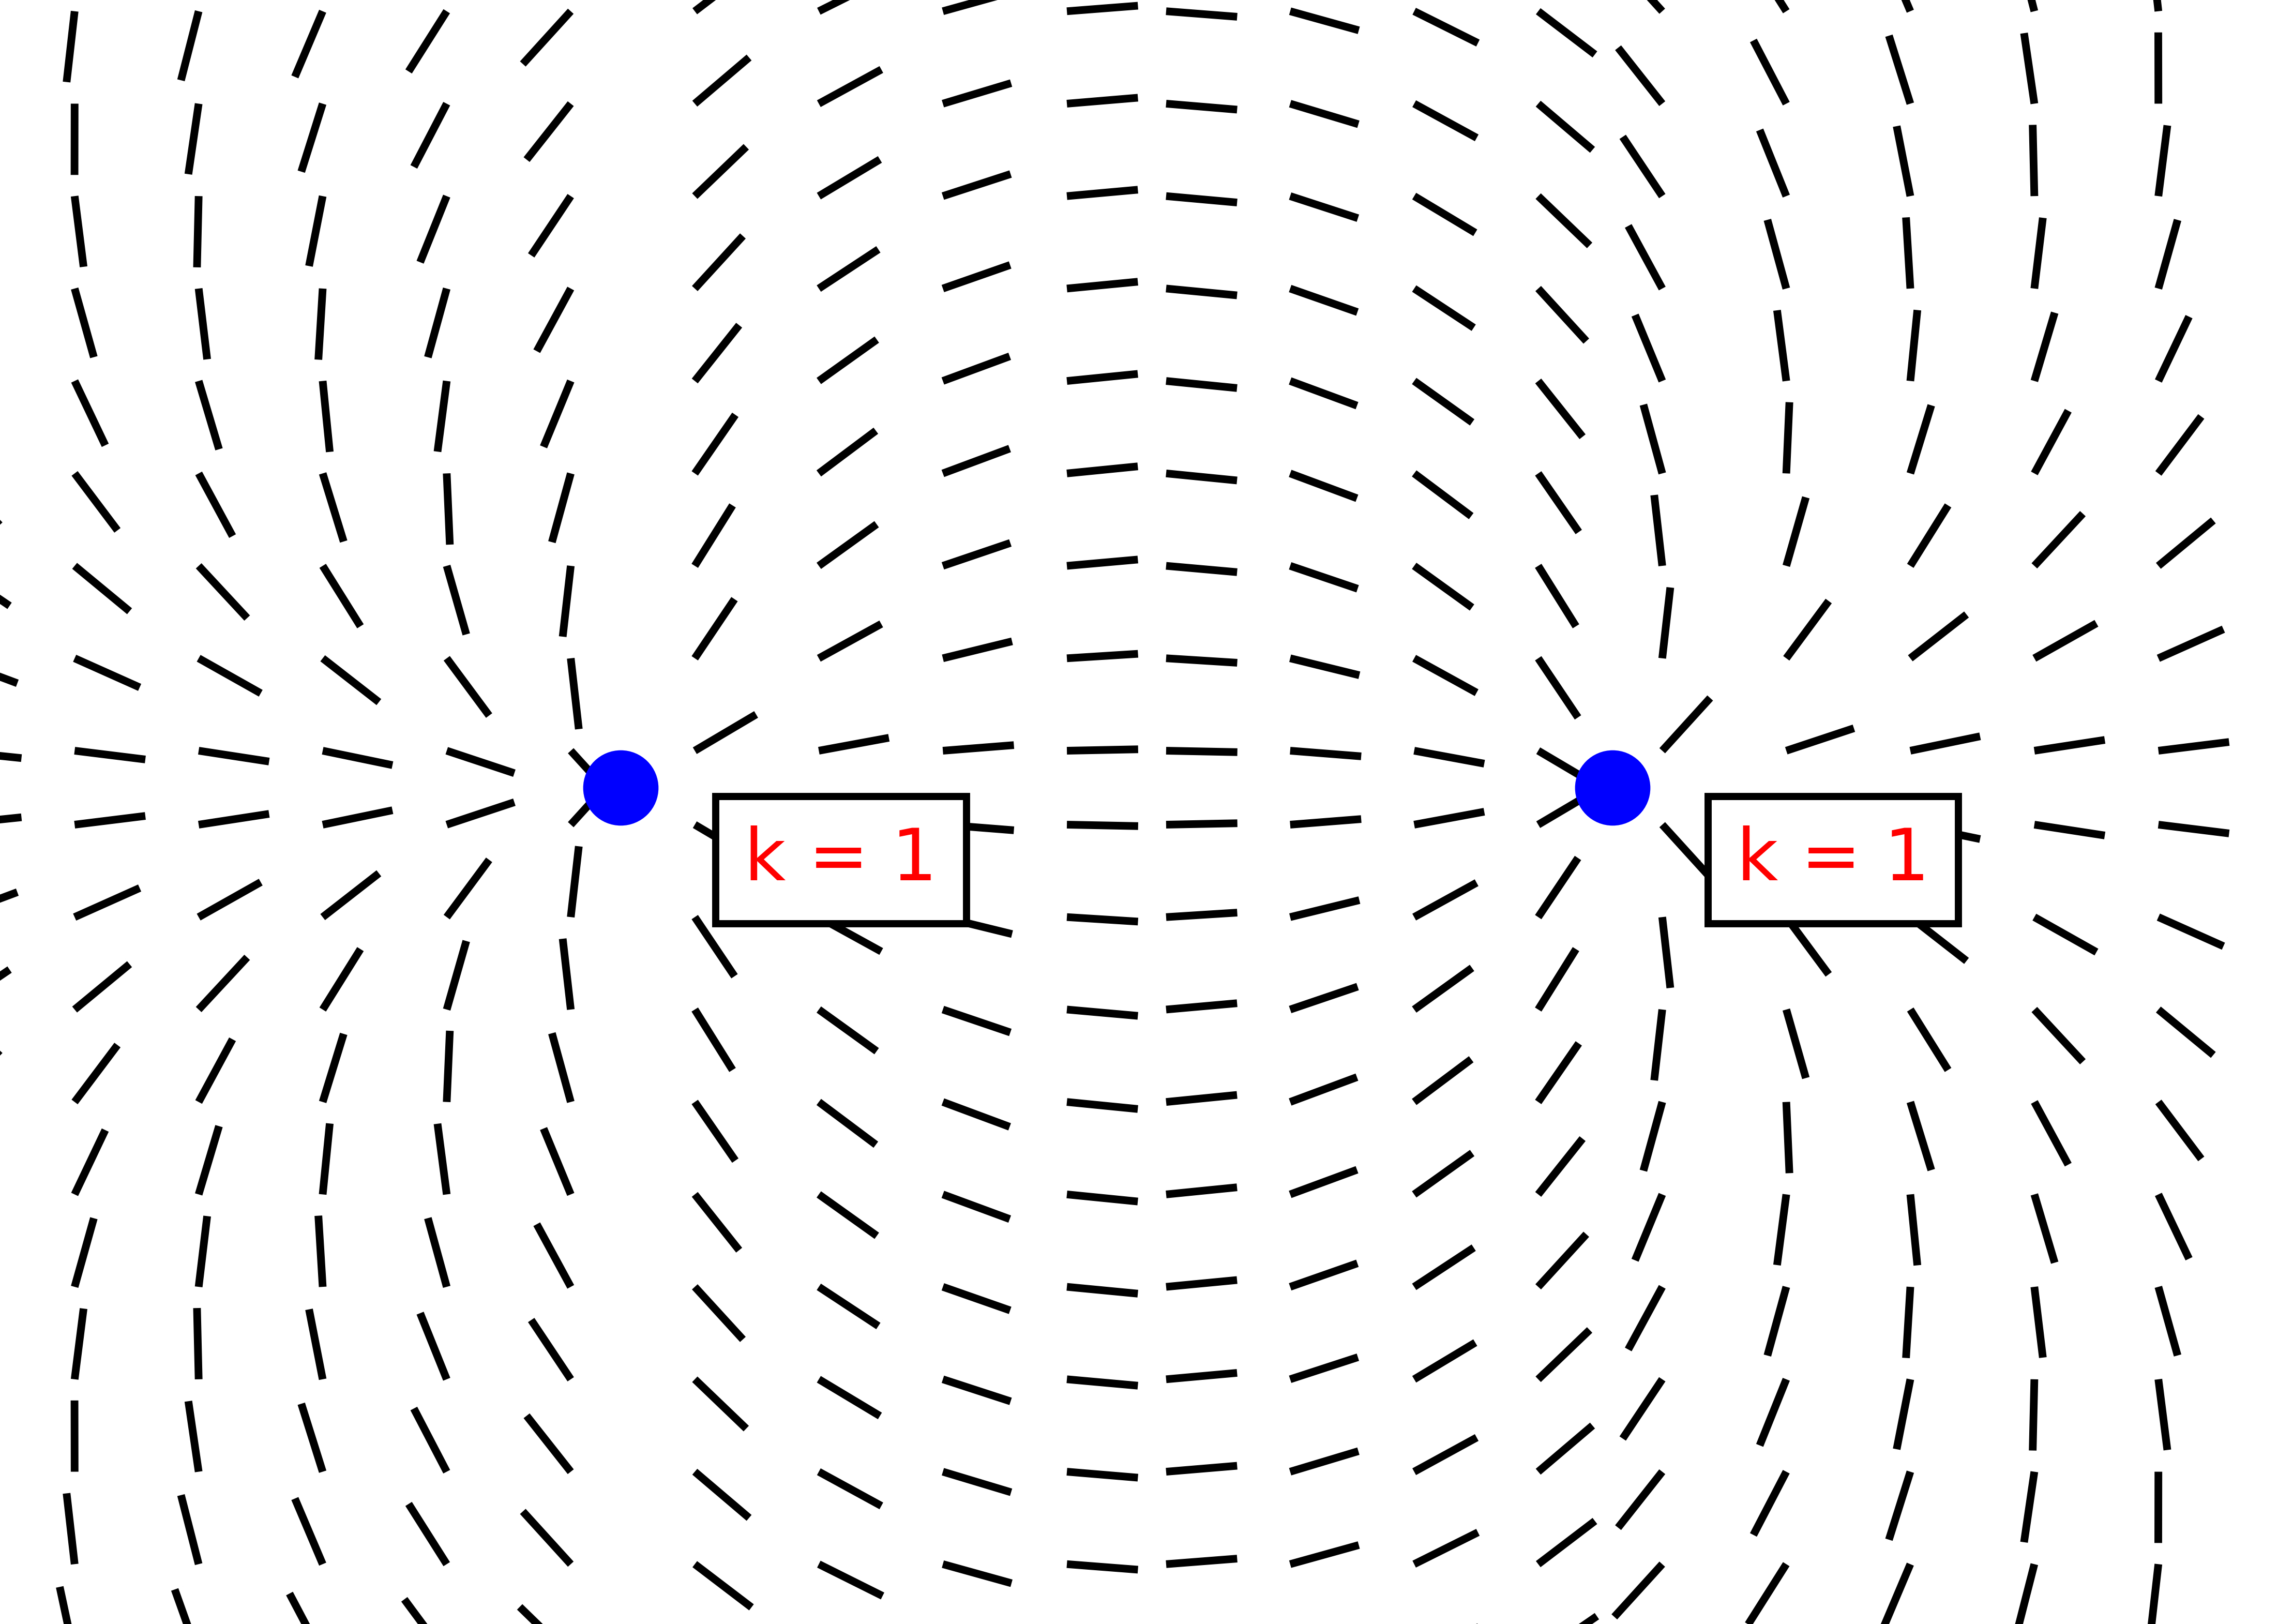
\includegraphics[width=\textwidth]{orient_dva_11_crop.png}} % textwidth znotraj subfigure je tisti ki ga specifiramo na začetku subfigure (0.4 \textwidth)
        \caption{}
        \label{fig:dva}
    \end{subfigure}
    \hspace{1cm}
    \begin{subfigure}[b]{0.45\textwidth}
        \fbox{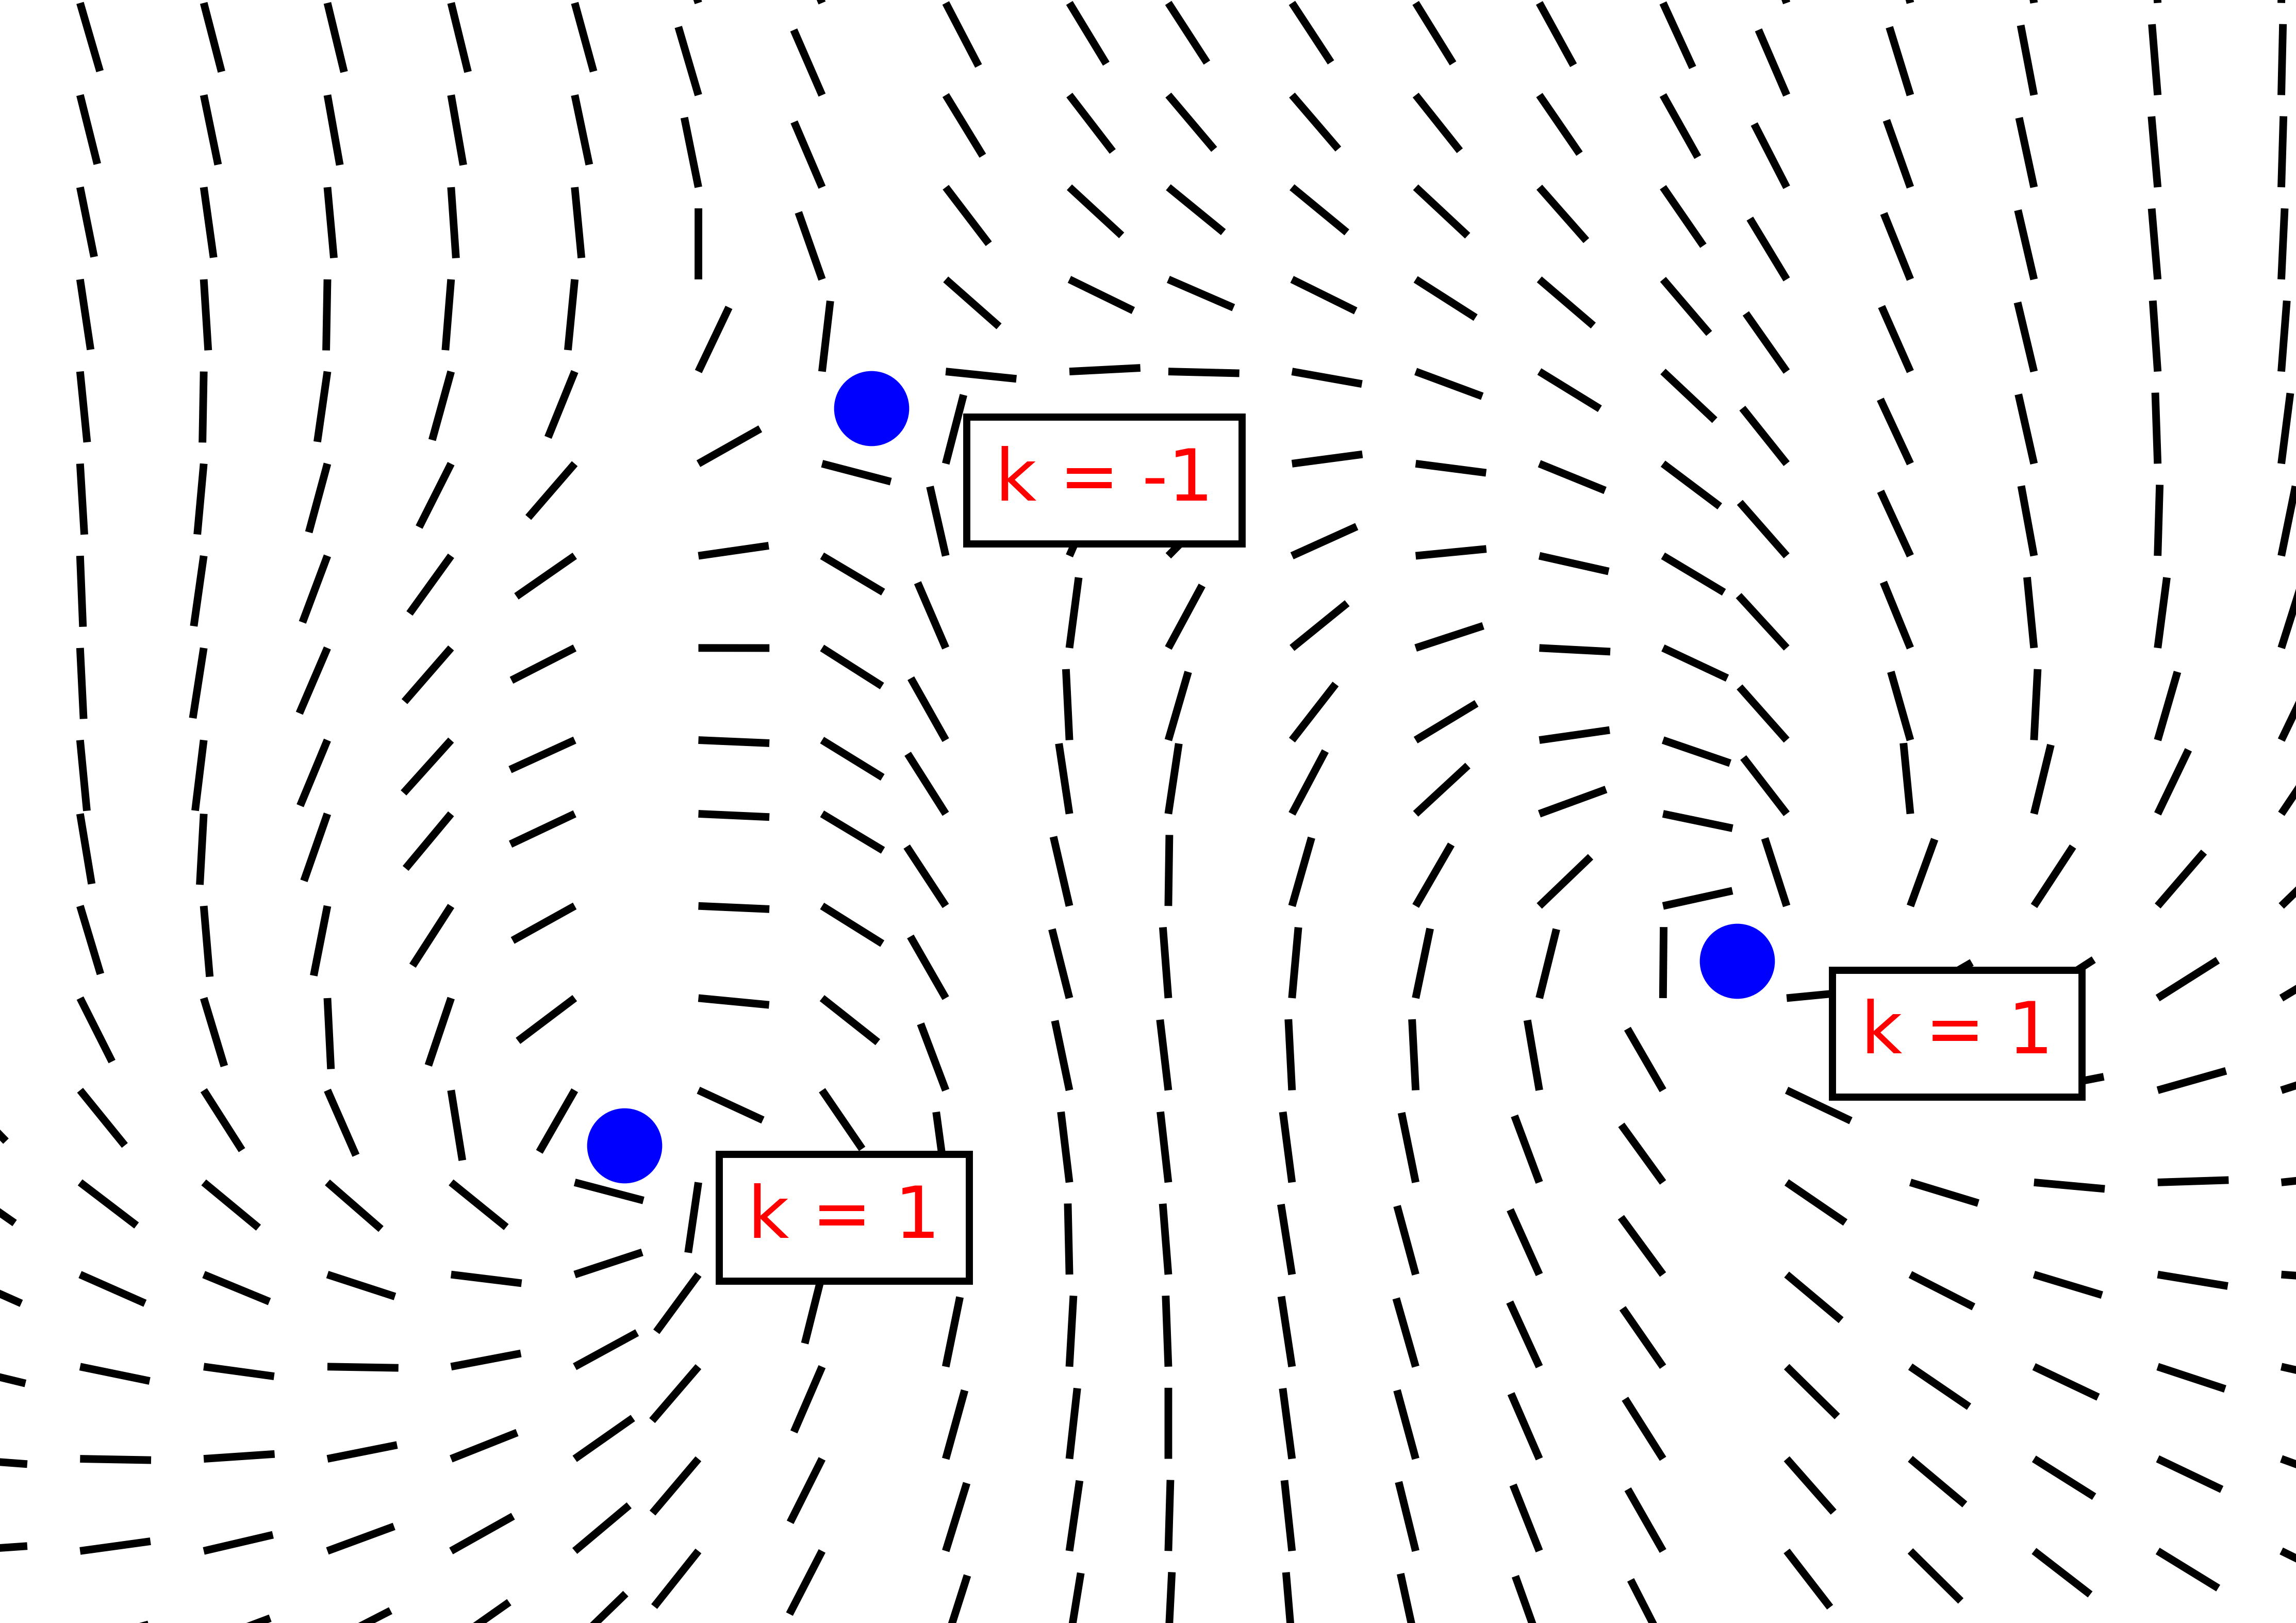
\includegraphics[width=\textwidth]{orient_tri_11-1_crop.png}} % textwidth znotraj subfigure je tisti ki ga specifiramo na začetku subfigure (0.4 \textwidth)
        \caption{}
        \label{fig:tri}
    \end{subfigure}
    \caption{Direktorsko polje dveh (a) in treh defektov (b). Modre pike so defekti, ovojna števila vsakega defekta pa so pripisana rdeče.}
    \label{fig:direktorsko}
\end{figure}
%\end{comment}


\section{Energija defektov}
Energijo defektov v tekočem kristalu lahko razdelimo na dva dela: (1) energijo jedra defekta in (2) elastično energijo \cite{chaikin1995principles}. Energija jedra je povezana s pokvarjeno orientacijo v jedru defekta in je v tej nalogi ne obravnavamo. Elastična energija je povezana z deformacijo direktorskega polja. V naslednjih razdelkih bomo videli, da tipično sestoji iz prispevkov energije vsakega defekta in prispevkov interakcijske energije med defekti \cite{chaikin1995principles}. V splošnem se energija defektov v 2D tekočem kristalu izračuna \cite{chandrasekhar1986structure} z
\begin{equation}
\label{eq:energija_splosno}
    E = \iint \left|\grad\phi\right|^{2}\,dS.
\end{equation}


\section{En defekt}
\label{sec:en}
Orientacijsko polje enega defekta se izraža kot
\begin{equation}
\label{eq:phi_kart_en}
    \phi=k_1 \arctan\left(\frac{y-y_{1}}{x-x_{1}}\right).
\end{equation}
Za izračun energije izberimo izhodišče koordinatnega sistema tako, da je defekt v izhodišču, in uporabimo polarne koordinate. Najprej se izraz (\ref{eq:phi_kart_en}) poenostavi v
\begin{align}
    \phi&=k_1 \arctan(\tan(\varphi)) \nonumber \\
    &= k_1 (\varphi + n\pi)\hspace{2cm}   n = 0,1, ... \nonumber
\end{align}
Gradient skalarnega polja $f$ se v polarnih koordinatah izraža kot
\begin{equation*}
    \grad f = \frac{\partial f}{\partial r}\bm{\hat{e}_{r}} + \frac{1}{r}\frac{\partial f}{\partial \theta}\bm{\hat{e}_{\theta}},
\end{equation*}
torej je
\begin{equation*}
    \grad \phi(r, \theta) = \frac{k_1}{r}\bm{\hat{e}_{\theta}}.
\end{equation*}
Za en defekt je torej energija
\begin{align}
    E &= \iint \left|\grad\phi\right|^{2}r\,dr\,d\varphi \nonumber \\
    &= k_{1}^{2}\int_{0}^{2\pi}\int_{\epsilon}^{R} \frac{1}{r} \,dr\,d\varphi \nonumber \\
    &= 2\pi k_{1}^{2} \ln{\frac{R}{\epsilon}}. \label{eq:energija_en}
\end{align}
%Tu je $R$ izbrana maksimalna velikost sistema, ponavadi tako, da je $\epsilon \ll R$ \cite{chandrasekhar1986structure}.
V integralu po $r$ je treba izbrati končno zgornjo in spodnjo mejo, sicer integral divergira. To naredimo tako, da za spodnjo mejo vzamemo radij jedra defekta $\epsilon$, za zgornjo pa maksimalno velikost sistema $R$, ponavadi tako, da je $\epsilon \ll R$ \cite{chandrasekhar1986structure}.
Izraz (\ref{eq:energija_en}) predstavlja energijo defekta v tekočem kristalu; to je elastična energija, ki je potrebna za uvedbo izoliranega defekta v tekoči kristal \cite{chandrasekhar1986structure}. V neskončnem sloju ($R \to \infty$) bi defekt moral imeti neskončno energijo, vendar se to v praksi ne zgodi zaradi prisotnosti parov defektov z nasprotnim ovojnim številom \cite{chandrasekhar1986structure}. Nastanek defektov z velikimi ovojnimi števili je energetsko neugoden, saj elastična energija raste s $k^{2}$ \cite{andrienko2018introduction}. 



%rc dosti manjsi od r12 dosti manjsi od r glej screenshot fundamentals shri singh

%kjer je $R$ zgornja končna meja (ang. \emph{cutoff radius} ~cite{}), $\epsilon$ pa jedro defekta. Ti dve količini sta vpeljani zato, da lahko izvrednotimo integral, ki bi sicer v mejah od $0$ do $\inf$ divergiral.



\section{Dva defekta}
\label{sec:dva}
Poglejmo si sedaj energijo dveh defektov. Tu je bolje uporabiti drugačen pristop, ki se lažje posploši na izračun interakcijske energije med defektoma in je uporabljen v (Chaikin et al., 1995 \cite{chaikin1995principles}).
Obravnavajmo s tem pristopom najprej en izoliran defekt. Orientacijsko polje $\phi$ je podano z izrazom (\ref{eq:phi_kart_en}) in se nezvezno spremeni za $2\pi k$ vsakič, ko prečka pozitivni del x osi v nasprotni smeri urinega kazalca. Pri tem je $k$ ovojno število defekta. Os x si lahko zato predstavljamo kot \emph{rez}, ki ustvari dve namišljeni površini $\Sigma^{+}$ in $\Sigma^{-}$ (poltraka), prikazani na sliki \ref{fig:rez}. Na vsaki površini ima $\phi$ konstantno vrednost; na $\Sigma^{-}$ je $\phi = 0$, na $\Sigma^{+}$ pa $\phi = 2\pi k$. Ta rez je samo matematični pripomoček in nima fizikalnega pomena.

\begin{figure}[H]
    \centering
    \includegraphics[width=0.9\textwidth]{rez2_crop.png}
    \caption{Rez (prirejeno po skici iz (Chaikin et al., 1995 \cite{chaikin1995principles}))}
    \label{fig:rez}
\end{figure}

\begin{comment}
$\bm{***}$ Za izračun energije bomo potrebovali izraz za integracijo po delih. Tega izpeljemo iz naslednjega pravila za odvod produkta:
\begin{equation*}
    \grad \cdot (f\grad g) = \grad f \cdot \grad g + f \grad^{2}g,
\end{equation*}
torej je
\begin{equation*}
    \iint \grad f \cdot \grad g \, dS  =  \iint \grad \cdot (f\grad g) \, dS - \iint f \grad^{2}g \, dS,
\end{equation*}

Prvi člen na desni strani lahko preoblikujemo z integralskim izrekom o divergenci $\iint_{\Omega} \bm{F} \,dS = \oint_{\partial \Omega} \bm{F} \cdot \bm{\hat{n}} \, dl$, tako da dobimo
\begin{equation*}
    \iint \grad f \cdot \grad g \, dS=  \int \grad \cdot (f\grad g) \bm{\hat{n}}\, dl - \iint f \grad^{2}g \, dS,
\end{equation*}
kar je ravno prva Greenova identiteta. $\bm{***}$
\end{comment}

\vspace{1cm}
\noindent Sedaj integriramo izraz za energijo (\ref{eq:energija_splosno}) po delih:
\begin{equation*}
    \iint \left(\grad\phi\right)^{2}\,dS = \iint \grad \cdot \left(\phi \grad\phi\right)\,dS - \iint \phi \left(\grad^{2}\phi\right) \, dS.
\end{equation*}
Drugi člen na desni je enak $0$, ker je $\phi$ harmonična, prvi člen pa preoblikujemo s pomočjo Stokesovega izreka in izreka o divergenci in dobimo
\begin{align}
    E = \iint \left(\grad\phi\right)^{2}\,dS &=\int \phi^{+}\left(\grad\phi\right)\bm{n}^{+} \, dr + \int \phi^{-}\left(\grad\phi\right)\bm{n}^{-} \, dr \nonumber\\
    &=\left(\phi^{+} - \phi^{-}\right) \int \left|\grad\phi\right| \, dr \label{eq:druga_vrstica} \\
    &=2\pi k \int_{\epsilon}^{R} \frac{k}{r} \, dr \nonumber \\
    &=2\pi k^{2} \ln{\frac{R}{\epsilon}}, \label{eq:energija_en_drugi_nacin}
\end{align}
kjer je $\phi^{+} = 2k\pi$, $\phi^{-} = 0$, $\bm{n}^{+}$ enotska normala na površino $\Sigma^{+}$ (pravokotno na $d\bm{r}$), $\bm{n}^{-}$ pa enotska normala na $\Sigma^{-}$ . Pri prehodu v drugo vrstico (\ref{eq:druga_vrstica}) smo upoštevali, da sta na območju reza vektorja $\grad \phi$ in $\bm{n}$ vzporedna. Normala $\bm{n}^{+}$ namreč kaže v smeri $\bm{\hat{e}}_{\varphi}$, normala $\bm{n}^{-}$ pa v smeri $-\bm{\hat{e}}_{\varphi}$. Izraz (\ref{eq:energija_en_drugi_nacin}) je enak izrazu, ki smo ga dobili v poglavju \ref{sec:en}.

Energija dveh defektov se lahko izračuna na podoben način. Orientacijsko polje dveh defektov v tekočem kristalu se izraža kot 
\begin{align}
    \phi&=k_1 \arctan\left(\frac{y-y_{1}}{x-x_{1}}\right) + k_2 \arctan\left(\frac{y-y_{2}}{x-x_{2}}\right) \nonumber \\
    &=: \phi_{1} + \phi_{2}. \nonumber
\end{align}
Tedaj je energija
\begin{align}
    E &= \iint \left(\grad\phi_{1} + \grad\phi_{2}\right)^{2}\,dS \nonumber \\
    &=E_1 + E_2 + \iint \grad\phi_{1} \grad\phi_{2} \, dS +  \iint \grad\phi_{2} \grad\phi_{1} \,dS. \label{eq:energija_vmes}
\end{align}
Prispevka $E_{1}$ in $E_{2}$ v (\ref{eq:energija_vmes}) sta prispevka vsakega defekta posebej in sta oblike kot v (\ref{eq:energija_en}). Pri tem smo aproksimirali $\epsilon \ll r_{12} \ll R$, kjer je $r_{12} = \left|\bm{r_{12}}\right| = \left|\bm{r_{2}}-\bm{r_{1}}\right|$ razdalja med defektoma. Ta aproksimacija zagotavlja, da sta v primerjavi z dimenzijo sistema $R$ jedri obeh defektov približno točkasti in da se oba defekta nahajata približno v izhodišču. Zato lahko za "lastni" prispevek energije vsakega defekta uporabimo kar rezultat (\ref{eq:energija_en}), le z drugim ovojnim številom. Zadnja dva integrala v (\ref{eq:energija_vmes}) sta prispevka interakcijske energije in sta enaka, a ju pišemo tako, ker sedaj napravimo per partes na dva različna načina (za vsak integrand posebej). Postopamo podobno kot v enačbi (\ref{eq:druga_vrstica}). Prvi integral se izračuna kot
\begin{align}
    \iint \grad\phi_{1} \grad\phi_{2} \, dS &= \iint \grad \cdot \left(\phi_{1}\grad\phi_{2}\right) \,dS - \iint \phi_{1}\left(\grad^{2}\phi_{2}\right) \,dS \nonumber \\
    &=(\phi_{1}^{+} - \phi_{1}^{-}) \int \left|\grad\phi_{2}\right| \, dr \nonumber \\
    &=2\pi k_{1} \int_{r_{12}}^{R} \frac{k_{2}}{r} \, dr \nonumber \\
    &=2\pi k_{1} k_{2} \ln{\frac{R}{r_{12}}}. \nonumber
\end{align}
Drugi integral je podoben, le zamenjamo indeksa in dobimo isti rezultat.
%mogoce je fora teh DVEH integralov to da pokaze da je vseeno po katerem delas per partes. ker data isto.
Tako dobimo končni rezultat
\begin{align}
    E&=E_1 + E_2 + 4\pi k_{1} k_{2} \ln{\frac{R}{r_{12}}} \nonumber \\
    \Aboxed{E&=2\pi (k_{1} + k_{2})^{2} \ln{\frac{R}{\epsilon}} + 4\pi k_{1}k_{2}\ln{\frac{\epsilon}{r_{12}}}}.
\end{align}
V zadnji vrstici smo v prvem členu skombinirali vse člene, odvisne od $R$ (seštevanje in odštevanje logaritmov).

\noindent
Sila med defektoma je tako
\begin{equation*}
    \boxed{\bm{F_{12}} = -\grad E_{12} = -4\pi k_{1}k_{2}\frac{\bm{r_{12}}}{r_{12}^{2}}},
\end{equation*}
kjer je $\bm{r_{12}} = \bm{r_{2}}-\bm{r_{1}}$ radij vektor, ki kaže od prvega k drugemu defektu.


Interakcijska energija med defektoma je analogna Coulombski elektrostatski energiji \cite{vromans2016orientational}, le odvisnost od razdalje med nabojema je tu drugačna: logaritemska za energijo, $1/r$ za silo, v primerjavi z $1/r$ odvisnostjo Coulombske energije in $1/r^{2}$ odvisnostjo sile med električnima nabojema. Defekta z nasprotno predznačenima ovojnima številoma (nabojema) se privlačita, defekta z enako predznačenima pa odbijata. 

Zanimivo je, da po anihiliaciji dveh defektov, ki imata nasprotni naboj velikosti ena, za njima ne ostane noben defekt \cite{liang2021phase}.
 Če se anihilirata defekt s celim nabojem in defekt s polštevilskim nabojem, je tudi končni naboj polštevilski \cite{liang2021phase}.

%Zanimivo je, da ko se defekta z nasprotnima nabojema velikosti ena premakneta drug proti drugemu in se anihilirata, izgineta in ni več nobenega izmed njiju \cite{liang2021phase}.


\section{Več defektov}

V primeru večih defektov se rezultat iz razdelka \ref{sec:dva} ustrezno posploši na več defektov.
\noindent Orientacijsko polje večih točkastih defektov v ravnini je
\begin{equation*}
    \phi=\sum_{i} \phi_{i} = \sum_{i} k_i \arctan\left(\frac{y-y_{i}}{x-x_{i}}\right).
\end{equation*}
Za energijo dobimo
\begin{equation*}
    E = \sum_{i}2\pi k_{i}^{2} \ln{\frac{R}{\epsilon}} + \mathop{\sum_{i,j}}_{j>i}4\pi k_{i}k_{j} \ln{\frac{R}{r_{ij}}},
\end{equation*}
sila i-tega defekta na j-ti defekt pa je
\begin{equation*}
    \bm{F_{ij}} = -\grad E_{ij} = -4\pi k_{i}k_{j}\frac{\bm{r_{ij}}}{r_{ij}^{2}},
\end{equation*}
kjer je $\bm{r_{ij}} = \bm{r_{j}}-\bm{r_{i}}$ radij vektor, ki kaže od i-tega k j-temu defektu.








%\section{Komentar}
%Opomba: V literaturi (npr. \cite{chaikin1995principles, tang2017orientation}) se pri izračunu energije defektov pred integralom pojavi še konstantni faktor $K/2$, kjer je $K$ Frankova elastična konstanta. V splošnem je gostota proste energije v nematskem tekočem kristalu sestavljena iz treh členov, ki vsak predstavlja svoj tip deformacije in mu pripada svoja Frankova konstanta $K_i$. Pogosto so te tri konstante približno istega reda velikosti, zato se v računih naredi "aproksimacijo ene konstante"; tj. da so vse tri konstante enake $K$, s čimer se poenostavi račun \cite{kleman2003soft}.

%Opomba: V tej nalogi so defekti obravnavani kot točkasti. Sicer je defektom možno še pripisati orientacijo (orientacijo njih samih), kar k energiji doda še dodaten člen, med defekti pa zaradi tega delujejo še navori \cite{de1993physics, tang2017orientation, missaoui2020annihilation}.

\begin{comment}
 \noindent Rezultati za interakcijsko energijo točkastih defektov se v različnih člankih in literaturi med seboj nekoliko razlikujejo \cite{tang2017orientation, chandrasekhar1986structure, simoes1991liquid, de1993physics}, saj so avtorji uporabili različne metode. V tej nalogi sem se za računanje interakcijske energije zgledoval po pristopu v (Chaikin, \cite{chaikin1995principles}).    
\end{comment}

%\section{Energija defektov}
%V literaturi\cite{} se tipično zapiše gostoto energije preko Frank-Olseenovega zakona. Pri tem nastopajo trije členi, vsaj fizikalno predstavlja svoj pojav: splay, twist, ... V aproksimaciji "ene konstante" ($K_1=K_2=K_3=K$) se gostota energije izraža z $w(x, y)=|\grad\phi|^{2}$.










\section{Zaključek}
V tekočih kristalih se pojavljajo topološki defekti, ki predstavljajo območja, v katerih urejenost molekul ni dobro definirana. Točkastim defektom pripišemo ovojno število, ki pove, kolikokrat se direktorsko polje ovije okoli defekta. Z uvedbo defektov v tekoči kristal je povezana elastična energija. Defekti med seboj interagirajo, oblika interakcijske energije med točkastimi defekti pa je podobna Coulombski interakcijski energiji med električnimi naboji. Defekta z nasprotno predznačenima ovojnima številoma se privlačita, tista z enako predznačenima pa odbijata.







\newpage
\bibliography{Reference.bib}
\end{document}